\section{Data Acquisition}
\label{sec:chap_slam_data_acquisition}

In the following section, we first describe the robotic platform and sensors used to gather our place recognition dataset. We then describe in more details the dataset acquisition procedure and the resulting data.

\subsection{Robotic Platform}
The Husky A200 is a medium size (990 x 670 x 390 \SI{28}{\milli\meter}) \gls{ugv} developed by Clearpath Robotics~\cite{ClearpathWeb}. It is a rugged robot designed for all terrain conditions, therefore well suited for our experiments in forest. It uses a differential-drive skid steer allowing easy control and in place turns for our data acquisition.

\begin{itemize}
    \item 1 m/s
    \item Good payload aka strong motor = rough terrain and basically any sensors.
\end{itemize}
\begin{figure}
    \centering
    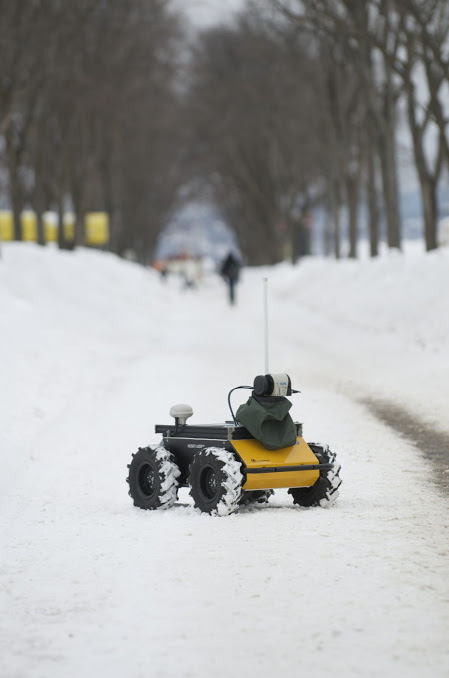
\includegraphics[width=0.95\linewidth]{img/chap_slam/husky.jpg}
    \caption{Wow such robot. \emph{Photo credit:} François Pomerleau}
    \label{fig:chap_slam_husky}
\end{figure}
\begin{table}[h]
    \begin{center}
        \caption{\label{tab:capteurs} Ensembles des capteurs du Husky A200 et du type de données associées.}
        \begin{tabular}{|c|c|c|}
            \hline
            \textbf{Capteur} & \textbf{Type de données} & \textbf{Précision et/ou}\\
                             &                          & \textbf{résolution} \\
            \hline
            \hline
            Caméra & Photo & 800x600 pixels\\
            \hline
            Capteur laser & Nuage de point & $\pm$ 0,04 mètre\\
                          & tridimensionnel & 0,25 degré\\
            \hline
            Centrale à inertie & Accélérations et & Inconnue\\
                                & vitesses angulaires & Inconnue\\
            \hline
            Courant des moteurs & Mesure du couple moteur & Inconnue\\
            \hline
            Encodeur des roues & Position angulaire des roues & 200000 impulsions\\
                               &                              &  par mètre\\
            \hline
            Système de positionnement & Coordonnées & 0,18 mètre\\
            mondial (GPS)             & géographiques & \\
            \hline
        \end{tabular}
    \end{center}
\end{table}

\subsection{Dataset}
\begin{figure}[htpb]
    \centering
    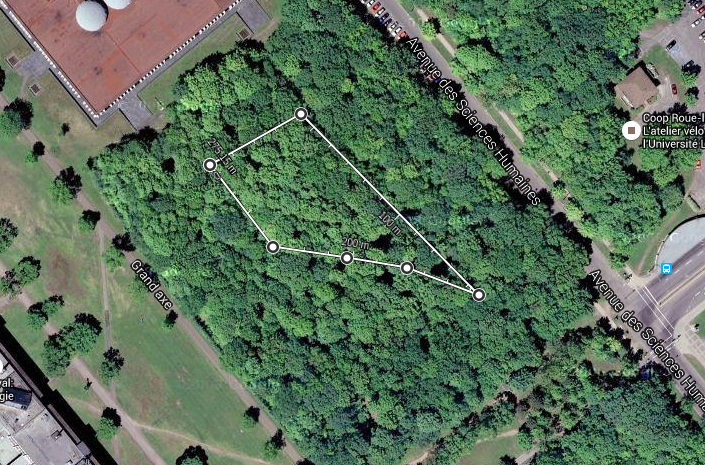
\includegraphics[width=0.95\linewidth]{img/chap_slam/path.png}
    \caption{Aerial view of the approximate path followed by the robot for data acquisition. Source: Google Maps, (2015)}
    \label{fig:chap_slam_path}
\end{figure}
